% !TEX root=/home/tavant/these/manuscript/src/manuscript.tex

\section{Axial Convection model}
  \label{sec-reinjectionnoise}
  \inlinenote{Add the section about reinjection noise.}

  As introduce in the previous section, the \ac{2D} radial-azimuthal simulation do not model a priori the convection.

  \subsection{Lafleur's model of injection}

    \citet{lafleur2016a} proposed a way to model the axial convection of the particles in a \ac{1D} purely azimuthal simulation.
    \Cref{fig-Fake_1d_1} shows a schematic illustration of the model.
    The principle is as follow
    \begin{itemize}
      \item We set a finite axial length, noted $L_z$ on \cref{fig-Fake_1d_1}.
      \item We follow the positions of the particle in the axial direction $z$
      \item When a particle crosses the boundary, it is removed.
      \item A new particle is created
      \begin{itemize}
        \item at $z=0$ for the ions
        \item  at $z=L_z$ for the electrons
      \end{itemize}
    \end{itemize}

    We create a new particle in order to conserve the charge in the simulation.
    The new particle has a velocity following a Maxwellian flux distribution function of a given temperature.
    The azimuthal position of the particle is chosen uniformly at random.

    \improvement{Add definition of the Maxellian and maxellian flux VDF ?}

    \begin{figure}[hbtp]
      \centering
      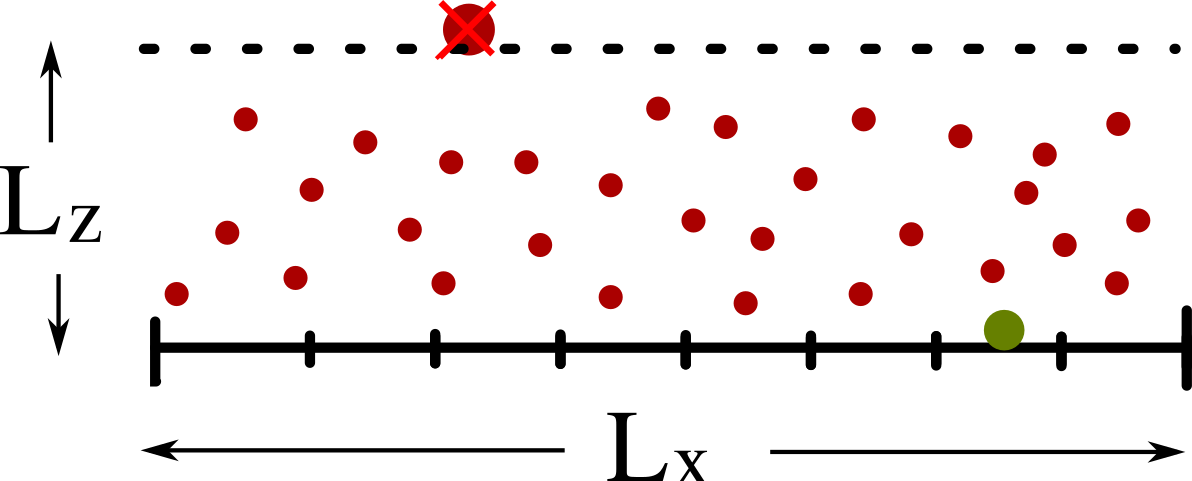
\includegraphics[width=\defaultwidth]{Fake_1d_2}
      \caption{Schematic representation of Trevor's convection model \citep{lafleur2016a}. The red particle is removed of the simulation, and the green particle is created. There, the particle is an ion. }
      \label{fig-Fake_1d_1}
    \end{figure}

    Lafleur's model of convection has been adopted in \ac{2D} by \citet{croes2017a}.
    The principle is exactly similar.
    The particles are followed in the 3 directions, and a finite length is used to close to axial direction.
    It is important to note that even is the particle are followed in the 3 directions, the meshed domain is only \ac{2D}.
    The simulation is not \ac{3D}-\ac{3V}.

    In \citet{croes2017a}, the authors have observed that if the newly created particle has a radial position chosen uniformly at random, it would affect the sheath.
    Hence, they decided to use the same radial position that the removed particle.
    \Cref{fig-Fake_2d} presents a schematic representation of the convection model in \ac{2D}.

    \begin{figure}[hbtp]
      \centering
      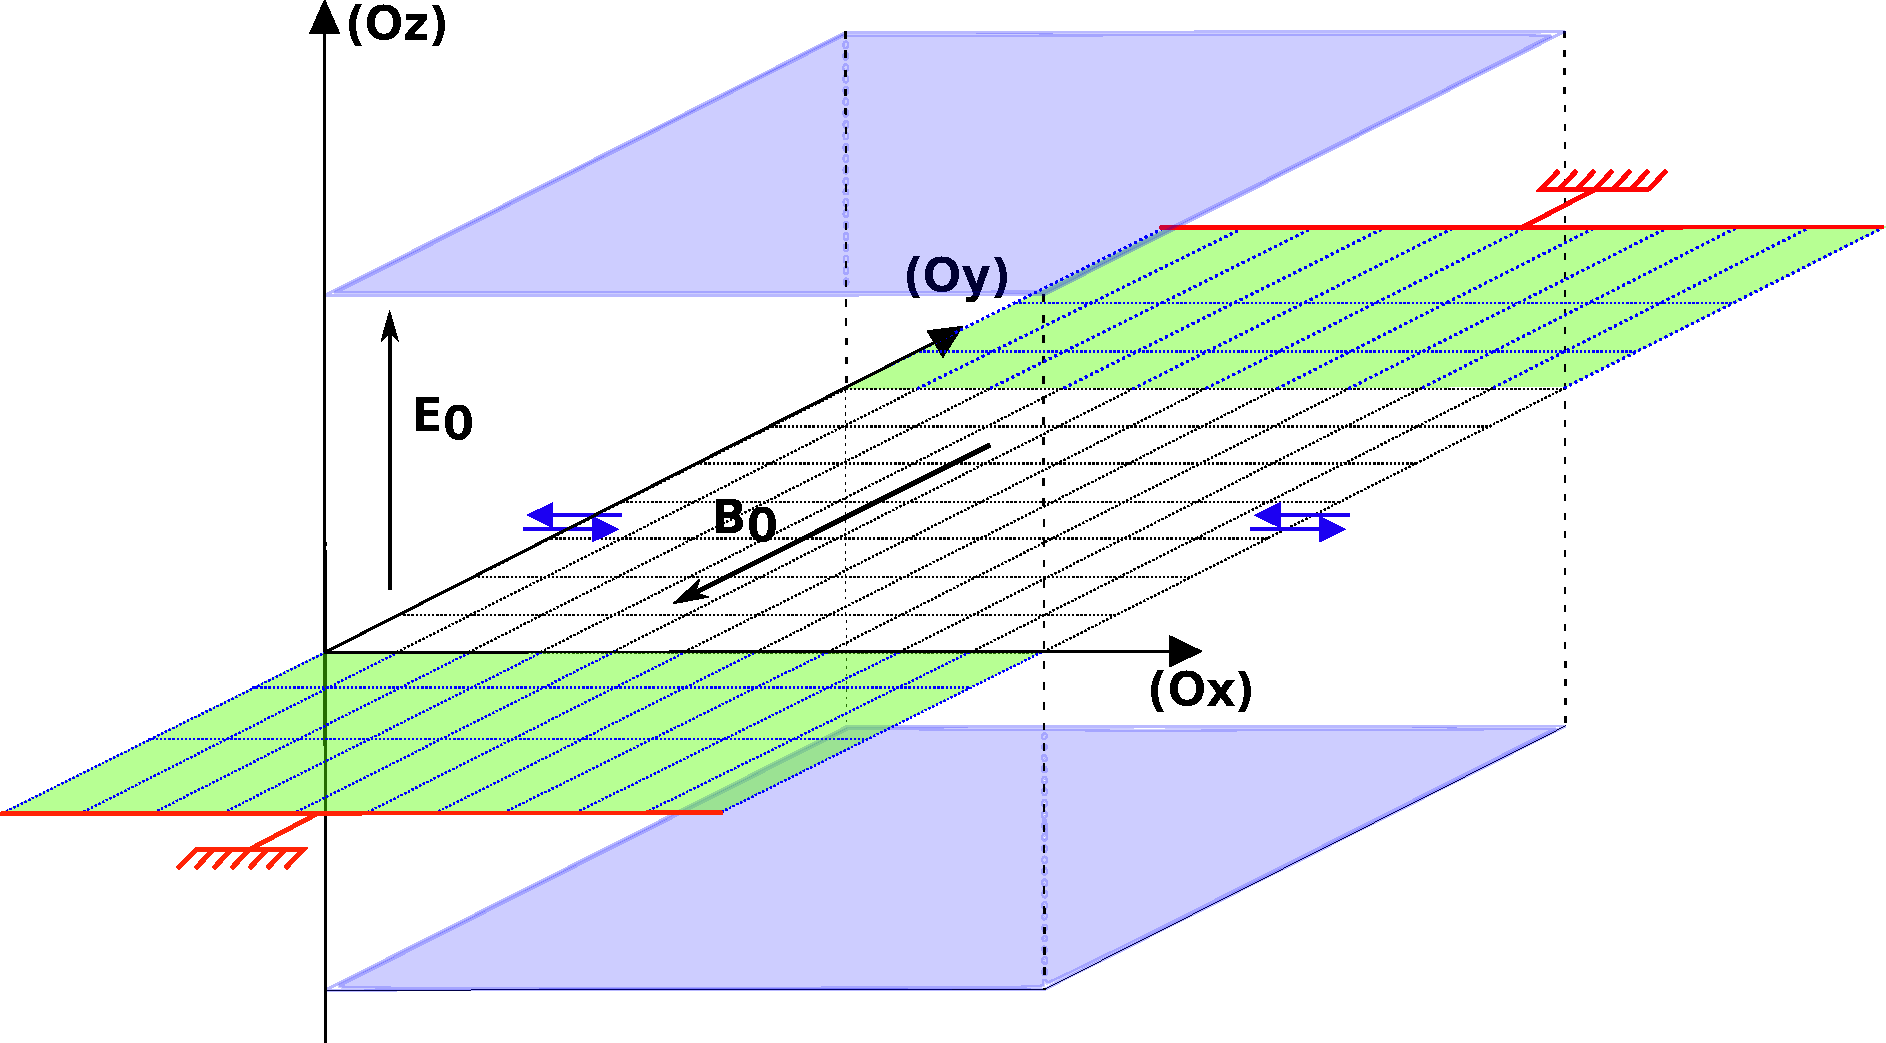
\includegraphics[width=\defaultwidth]{2_5D_dielectric_PPS_small}
      \caption{Schematic representation of the Lafleur's convection model adapted in \ac{2D}. The new particle radial position corresponds to the removed particle, but its azimuthal position is chosen uniformly at random. }
      \label{fig-Fake_2d}
    \end{figure}

    \Cref{fig-energy_convection} shows the evolution as a function of time of the electron mean energy in the simulation in a typical \ac{2D} radial-azimuthal simulation, addapted from \citet{croes2017}.
    We can see that without the convection, the mean energy quickly rises to unphysical values.
    When the convection is modeled, using an axial of $L_z=1$ cm, the energy reaches a steady state.
    \nomenclature[Q]{\ensuremath{ L_z}}{ Axial length}
    \begin{figure}[hbtp]
      \centering
      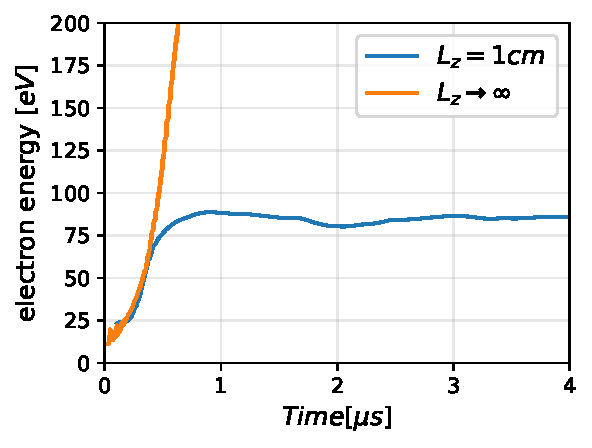
\includegraphics[width=\defaultwidth]{energy}
      \caption{Time evolution of the electron mean energy when the convection is not modeled ($L_z \rightarrow \infty$) and with Trevor's convection model used, $L_z = 1$ cm. Adapted from \citet{croes2017}.}
      \label{fig-energy_convection}
    \end{figure}



  \subsection{Numerical artefacts}
    \citet{lafleur2016a} studied the impact of the convection model on the simulation results.
    The authors observed in particular that changing the azimuthal length of the simulation domain could affect the simulation results.

    \Cref{fig-convection_numerical} shows the

    \begin{figure}[hbtp]
      \centering

      \begin{tabular}{cc}
        \subfigure{Lafleur_NoLz_1}{a}{20, 20}
            &
        \subfigure{Lafleur_Lz_1}{b}{20, 20} \\

        \subfigure{Lafleur_NoLz_2}{c}{20, 20} &
        \subfigure{Lafleur_Lz_2}{d}{20, 20} \\
      \end{tabular}
      \caption{Effects of Lafleur's convection model for two different azimuthal length on the azimuthal electric field. ({\bf a}) No convection, $L_x=0.5$~cm,  ({\bf b}) convection modeled, $L_x=0.5$~cm,  ({\bf c}) No convection, $L_x=1$~cm,  ({\bf d}) convection modeled, $L_x=1$~cm. The colour of each plots is normalized to the maximum amplitude. Adapted from \citep{lafleur2016a}.}
      \label{fig-convection_numerical}
    \end{figure}
